\documentclass[12pt]{article}
\usepackage[margin=2.5cm]{geometry}
\usepackage{enumerate}
\usepackage{amsfonts}
\usepackage{amsmath}
\usepackage{fancyhdr}
\usepackage{amsmath}
\usepackage{amssymb}
\usepackage{amsthm}
\usepackage{mdframed}
\usepackage{graphicx}
\usepackage{subcaption}
\usepackage{adjustbox}
\usepackage{listings}
\usepackage{xcolor}
\usepackage{courier}
\usepackage[utf]{kotex}
\usepackage{hyperref}
\usepackage{soul}
\usepackage{cancel}


\definecolor{codegreen}{rgb}{0,0.6,0}
\definecolor{codegray}{rgb}{0.5,0.5,0.5}
\definecolor{codepurple}{rgb}{0.58,0,0.82}
\definecolor{backcolour}{rgb}{0.95,0.95,0.92}

\lstdefinestyle{mystyle}{
    backgroundcolor=\color{backcolour},
    commentstyle=\color{codegreen},
    keywordstyle=\color{magenta},
    numberstyle=\tiny\color{codegray},
    stringstyle=\color{codepurple},
    basicstyle=\ttfamily\footnotesize,
    breakatwhitespace=false,
    breaklines=true,
    captionpos=b,
    keepspaces=true,
    numbers=left,
    numbersep=5pt,
    showspaces=false,
    showstringspaces=false,
    showtabs=false,
    tabsize=1
}

\lstset{style=mystyle}

\pagestyle{fancy}
\renewcommand{\headrulewidth}{0.4pt}
\lhead{CSC 369}
\rhead{Reading Notes}

\begin{document}
\title{CSC 369 Reading Notes}

\section{Process}

\begin{mdframed}
\underline{\textbf{Vocabularies}}

\bigskip

\begin{enumerate}[1.]
    \item \textbf{Process}
    \begin{itemize}
        \item Is a program in execution
    \end{itemize}
    \item \textbf{Running Program}
    \begin{itemize}
        \item Is a collection of coded software instructions that can be executed
        by a computer to perform a specific task
    \end{itemize}
    \item \textbf{Time Sharing}
    \begin{itemize}
        \item Is a basic technique used by an OS to share a resource
        \item Allows an entity to use the resource for a little while, and then
        a little while by another, and so forth

        \bigskip

        \underline{\textbf{Example}}

        \bigskip

        CPU

    \end{itemize}
    \item \textbf{Space Sharing}
    \begin{itemize}
        \item Is where a resource (space) is divided among those who wishes to use it

        \bigskip

        \underline{\textbf{Example}}

        \bigskip

        Disk, and Memory
    \end{itemize}
    \item \textbf{Mechanism}
    \begin{itemize}
        \item Is a low-level method or protocol that implement a needed piece of
        functionality.

        \bigskip

        \underline{\textbf{Example}}

        \bigskip

        Context Switching
    \end{itemize}
    \item \textbf{Policy}

    \begin{itemize}
        \item Is an algorithm for making some kinds of decision within the OS

        \bigskip

        \underline{\textbf{Example}}

        \bigskip

        Scheduling Policy. That is, what kind of program should the OS run?
    \end{itemize}
    \item \textbf{Address Space}
    \begin{itemize}
        \item Is a range of discrete addresses where each corresponds to a memory cell

        \bigskip

        \begin{center}
        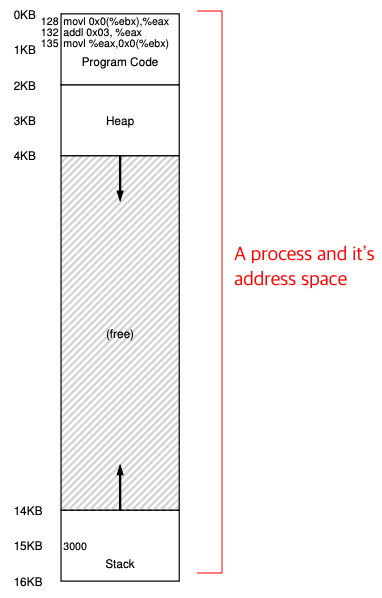
\includegraphics[width=0.5\linewidth]{images/notes_4_1.png}
        \end{center}

    \end{itemize}
    \item \textbf{Program Counter}
    \begin{itemize}
        \item Is also called \textbf{Instruction Pointer}
        \item Is a process register that tells which instruction of the program
        is currently being executed
    \end{itemize}
    \item \textbf{Stack Pointer}
    \begin{itemize}
        \item Is a resgister that points to the location of last item placed in memory block

        \begin{center}
        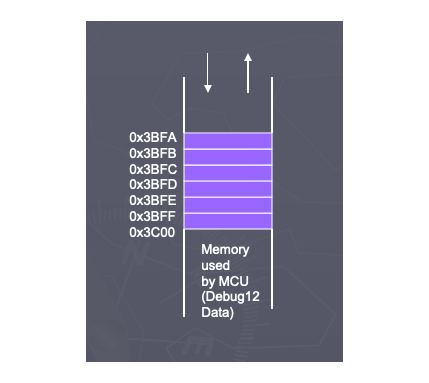
\includegraphics[width=0.5\linewidth]{images/notes_4_2.png}
        \end{center}
    \end{itemize}
    \item \textbf{Frame Pointer}
    \begin{itemize}
        \item Is a reference pointer allowing a debugger to know where local
        variable or an argument is at with a single constant offset

        \begin{center}
        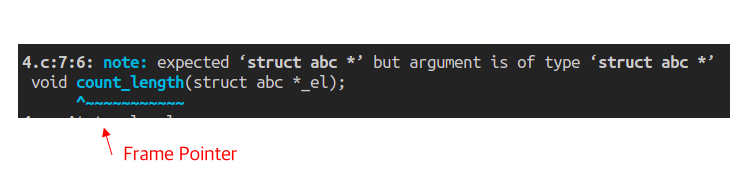
\includegraphics[width=0.8\linewidth]{images/notes_4_3.png}
        \end{center}
    \end{itemize}
    \item \textbf{Eager Loading Process}
    \begin{itemize}
        \item Is the process that loads all code and data before running the program
    \end{itemize}
    \item \textbf{Lazy Loading Process}
    \begin{itemize}
        \item Is the process that loads piece of code or data only as they are needed during
        program execution
    \end{itemize}
    \item \textbf{Stack}
    \begin{itemize}
        \item Is also called \textbf{runtime stack}, \textbf{automatic memory}
        \item Is a special region in computer's memory that temporarily stores local variables,
        function parameters, and return addresses
        \item Is managed by compiler
    \end{itemize}
    \item \textbf{Heap}
    \item \textbf{File Descriptors}
    \item \textbf{Persistence}
    \item \textbf{Process States}
    \item \textbf{Process List}
    \item \textbf{Context Switch}
    \item \textbf{Process Control Block}
    \item \textbf{Zombie State}
\end{enumerate}

\end{mdframed}

\end{document}
